\section{Derivations of Least Squares}
Least Squares regression solves an over-constrained set of equations as a minimization of the residuals squared($v_i$).  There are a few different least squares regression methods, which will be described in this section.

\[
min \sum_{i=1}^{n} v_i^2
\]

\subsection{Ordinary and Weighted Least Squares}
Ghalani provides a good basic example explanation of a simple ordinary least squares problem (Section 11.6.1 Ghalani). Consider the 3 equations provided below.  

\subsubsection*{Equations}
The system is overconstrained and there is no solution that satisfies each equation.
\begin{align*}
x+y &= 3.0 \\
2x-y &= 1.5 \\
x-y &= 0.2 \\
\end{align*}

\subsubsection*{Observation Equations}
In order to solve the solution, we add a \textit{residual} for each equation.  This residual captures any error in the measurements.  These equations are called the observation equations, and are a foundation of least squares.
\begin{align*}
x+y &= 3.0 + v_1\\
2x-y &= 1.5 + v_2\\
x-y &= 0.2 + v_3\\
\end{align*}

\subsubsection*{Residual Equations}
The observation equations can be rewritten as residual equations, shown below.	
\begin{align*}
v_1 &= x + y - 3.0 \\
v_2 &= 2x - y - 1.5 \\
v_3 &= x - y - 0.2 \\
\end{align*}

The goal of least squares is to determine a solution which minimizes the sum of the square of the residuals... or to get the \textbf{least squares solution!}

\[
min(\sum\limits_{i=1}^n v_i^2)
\]

\subsubsection*{Sum of Squares Equation}
\[
f(x,y) = (x+y-3.0)^2 + (2x-y-1.5)^2 + (x-y-0.2)^2
\]

The minimum of the sum of squares is where the derivative in the x and y dimension is equal to 0.  Therefore we derive a normal equation as the partial derivative with respect to each unknown variable, in this case (x,y).

\subsubsection*{Normal Equation Derivation}
\begin{align*}
\ddx{f(x,y)}{x} &= 2(x+y-3.0) + 2(2x-y-1.5)(2) + 2(x-y-0.2) \\
\ddx{f(x,y)}{y} &= 2(x+y-3.0) + 2(2x-y-1.5)(-1) + 2(x-y-0.2)(-1)
\end{align*}

\subsubsection*{Normal Equations}
\begin{align*}
6x-2y -6.2 &= 0 \\
-2x +3y -1.3 &= 0
\end{align*}
Solving for the normal equations yields the 'most probable solution'.
\subsubsection*{Solving Normal Equations Using Matrices}
\[
\begin{bmatrix}
6 & -2 \\ 
-2 & 3 \\
\end{bmatrix}
\begin{bmatrix}
x \\ y
\end{bmatrix}
= 
\begin{bmatrix}
6.2 \\ 1.3
\end{bmatrix}
\]
\[
\begin{bmatrix}
x \\ y
\end{bmatrix}
= 
inv\left(
\begin{bmatrix}
6 & -2 \\ 
-2 & 3 \\
\end{bmatrix}
\right)
\begin{bmatrix}
6.2 \\ 1.3
\end{bmatrix}
\]
\[
\begin{bmatrix}
x \\ y
\end{bmatrix}
= 
\begin{bmatrix}
1.514 \\ 1.443
\end{bmatrix}
\]
\subsubsection*{Derive Normal Equations Using Matrices}
If we write our initial observation equations as matrices...
\[AX = L + V
\]
\[
A = 
\begin{bmatrix}
1 & 1 \\ 2 & -1 \\ 1 & -1 
\end{bmatrix}
\hspace{1cm}
X = 
\begin{bmatrix}
x \\ y
\end{bmatrix}\\
\hspace{1cm}
L = 
\begin{bmatrix}
3.0 \\ 1.5 \\ 0.2
\end{bmatrix}
\hspace{1cm}
V = 
\begin{bmatrix}
v_1 \\ v_2 \\ v_3
\end{bmatrix}
\]
Pre-multiplying both sides of the equation by $A^T$, we get the same Normal Equations as above! (V goes away because the normal equation can be solved without residuals).  $A^TA$ is sometimes rewritten as $N$, or the Normal Matrix.
\begin{align*}
AX &= L + V \\
A^TAX &= A^TL \rightarrow \text{ sometimes written as } NX = A^TL\\
\begin{bmatrix}
1 & 2 & 1 \\ 1 & -1 & -1
\end{bmatrix}
\begin{bmatrix}
1 & 1 \\ 2 & -1 \\ 1 & -1 
\end{bmatrix}
\begin{bmatrix}
x \\ y
\end{bmatrix}
&=
\begin{bmatrix}
1 & 2 & 1 \\ 1 & -1 & -1
\end{bmatrix}
\begin{bmatrix}
3.0 \\ 1.5 \\ 0.2
\end{bmatrix} \\
\begin{bmatrix}
6 & -2 \\ 
-2 & 3 \\
\end{bmatrix}
\begin{bmatrix}
x \\ y
\end{bmatrix}
&= 
\begin{bmatrix}
6.2 \\ 1.3
\end{bmatrix}
\end{align*}
Notice that this is the same as the normal equations derived above.
\subsubsection*{Derive Matrix Least Squares Solution (Ordinary Least Squares)}
Putting the pieces together, we can now solve for the least squares solution using matrices where X represents the most probable values which are the result of a minimization of the squared residuals of each observation.
\begin{align*}
AX &= L + V \\
A^TAX &= A^TL \\
X &= inv(A^TA)A^TL
\end{align*}
\subsubsection*{Add a Weight Term (Stochastic Model)}
The weight matrix, W, is used to weight the importance of each observation equation.  This is used when you have higher confidence in certain observations, and want those observations to more significantly influence your result.  While these weights can be related to anything, it is most common in geomatics that the W matrix is equal to the covariance matrix for all of the observation equations.  Normally each observation is assumed to be statistically independent, which would yield a diagonal matrix with no covariances.  This is often refereed to as Weighted Least Squares(WLS).  However, in an example using GPS surveying, 3 observation equations (X,Y,Z) with covariances are created for each measurement.  When Covariances are present, this is often referred to as General Least Squares(GLS).  The equations to solve the system are exactly the same.  Note: Ghilani Textbook does not use the WLS-GLS nomenclature, as he describes GLS the same way others describe TLS online, so I've chosen to follow the "internet" method for this document.

An example weight matrix for 4 observations equations (a,b,c,d) is shown below for WLS and GLS.
\begin{align*}
\text{Weighted Least Squares(WLS) } W = \Sigma^{-1} &= 
\begin{bmatrix}
\sigma_{aa}^2 & 0 & 0 & 0 \\ 
0 & \sigma_{bb}^2 & 0 & 0 \\
0 & 0 & \sigma_{cc}^2 & 0 \\
0 & 0 & 0 & \sigma_{dd}^2 \\
\end{bmatrix}
^{-1}
=
\begin{bmatrix}
\dfrac{1}{\sigma_{aa}^2} & 0 & 0 & 0 \\ 
0 & \dfrac{1}{\sigma_{bb}^2} & 0 & 0 \\
0 & 0 & \dfrac{1}{\sigma_{cc}^2} & 0 \\
0 & 0 & 0 & \dfrac{1}{\sigma_{dd}^2} \\
\end{bmatrix}
\\
\text{General Least Squares(GLS) } W = \Sigma^{-1} &= 
\begin{bmatrix}
\sigma_{aa}^2 & \sigma_{ab}^2 & \sigma_{ac}^2 & \sigma_{ad}^2 \\ 
\sigma_{ab}^2 & \sigma_{bb}^2 & \sigma_{bc}^2 & \sigma_{bd}^2 \\ 
\sigma_{ac}^2 & \sigma_{bc}^2 & \sigma_{cc}^2 & \sigma_{cd}^2 \\ 
\sigma_{ad}^2 & \sigma_{bd}^2 & \sigma_{cd}^2 & \sigma_{dd}^2 \\ 
\end{bmatrix}
^{-1}
\end{align*}
\subsubsection*{Weighted Linear Least Squares and General Least Squares Equation}
Incorporating the Weight matrix results in the following, where $A^TWA$ is the Normal Matrix.
\begin{align*}
WAX &= WL + WV \\
A^TWAX &= A^TWL \\
X &= inv(A^TWA)A^TWL
\end{align*}

\subsection{Nonlinear Least Squares}
Each of the previous examples only considered linear observation equations, so the values in the A matrix were constants.  When this is not the case, an iterative nonlinear least squares approach must be used.  Instead of writing the observation equation as $AX=L+V$ as in the linear case, we write the observation equations as $JX=K+V$. Where J is a matrix of partial derivatives of each observation with respect to each unknown.  This method is based on taylor series expansion, and it requires a guess at the initial X ($X_0$).  

The X, in this case, is sometimes written as a $\Delta X$, as it represents a delta from the initial guess.  The delta is applied to the initial guess, and it a new delta is solved... which is then applied.  This iterative approach is performed until it stabilizes on a solution.  The exit criteria for the loop is normally based on when the reference variance $S_0^2$ increases.  This either means, your solution is diverging to a poor solution, or the deltas have become so small, that they are "bouncing" up and down about the solution.  Other exit criteria are a finite number of iterations, or a small absolute value of the delta values for each unknown.  Incorporating a maximum loop iterations is a good idea so that the while loop does not spin off into oblivion.  

\subsubsection*{Weighted Nonlinear Least Squares}
Incorporating the Weight Matrix results in the following nonlinear least squares solution.
\begin{align*}
WJ\Delta X&=WK+WV \\
J^TWJ\Delta X &= J^TWK \\
\Delta X &= inv(J^TWJ)J^TWK
\end{align*}
\subsection{Total Least Squares (TLS)}
*This section is derived from the "General Least Squares" section of Ghilani... From reading online, I believe this is actually called TLS by most other communities.  

It is important to recognize that the weight in all of the previous examples is associated with each observation equation, and not each individual variable.  For example, when solving a coordinate transformation, it is impossible to have error in both the reference and transformed coordinates. Total Least Squares is required to allow residuals in each of the variables.

Consider the least squares fit of a line with the observation equation to fit a linear line through a set of data points.  Notice that the residual is associated with the y coordinate.
\[
mx+b = y + v
\]

This is almost always the methodology performed when you do a linear regression with most software packages.  If, however, you want to have error in both the x and y coordinate, you must use TLS.  The observation equation would then be: 
\[
m(x+v_x) + b = (y + v_y)
\]

A visual plot showing how the fit from TLS is different is shown below:
\begin{figure}[H]
	\centering
	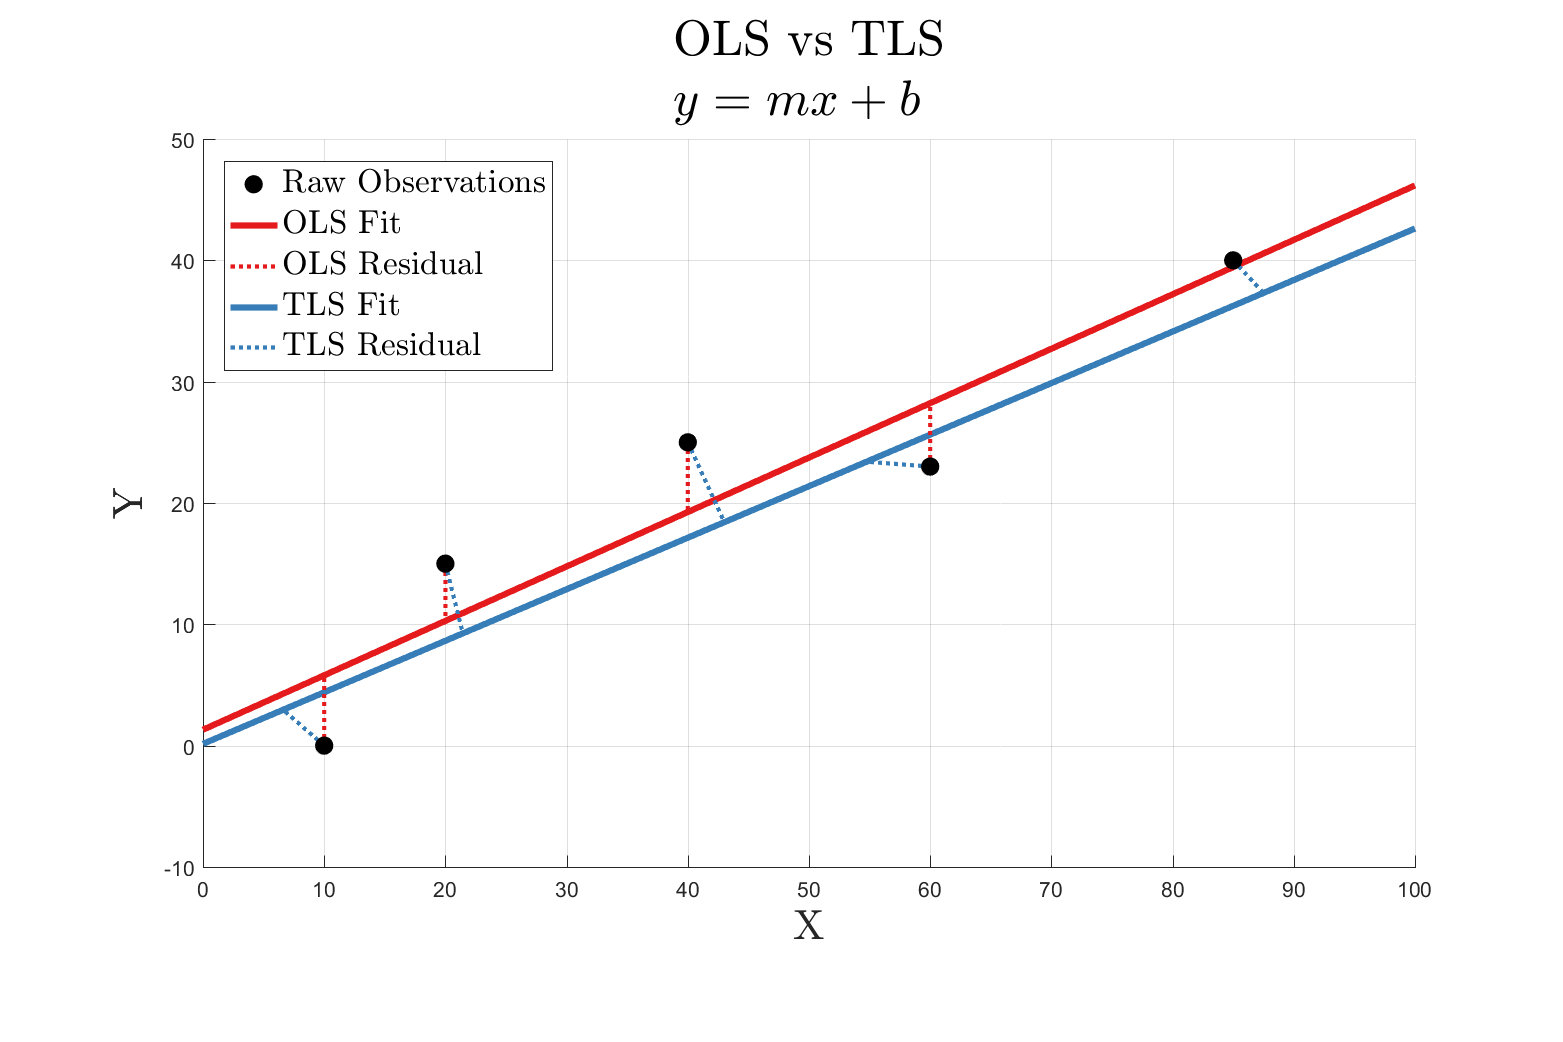
\includegraphics[height = 4in]{TLSexampleB.png}
\end{figure}

\subsubsection*{Total Least Squares Solution}
Define your observation equations such that all of the observations and residuals are on the left side of the equation.

\begin{align*}
mx + b &= y \\
m(x+v_x) + b &= (y+v_y) \\
m(x+v_x) + b - (y+v_y) &= 0 \\
\end{align*}

Now we want to linearize the equation with respect to the unknowns and the observations.  
\[
F: m(x+v_x) + b - (y+v_y) = 0
\]

\begin{align*}
\ddx{F}{x}v_x + \ddx{F}{y}v_y + \ddx{F}{m}d_m + \ddx{F}{b}d_b &= 0 - (m_0x+b_0-y) \\
mv_x -v_y + xd_m + d_b &= 0 - (mx+b-y) \\
\end{align*}

Now if we had 4 points (A,B,C,D), we could write the following equations.

\begin{align*}
mv_{x_A} -v_{y_A} + x_Ad_m + d_b &= 0 - (mx_A+b-y_A) \\
mv_{x_B} -v_{y_B} + x_Bd_m + d_b &= 0 - (mx_B+b-y_B) \\
mv_{x_C} -v_{y_C} + x_Cd_m + d_b &= 0 - (mx_C+b-y_C) \\
mv_{x_D} -v_{y_D} + x_Dd_m + d_b &= 0 - (mx_D+b-y_D) \\
\end{align*}

Which can be rewritten in Matrix form:

\[
BV + JX = K
\]

Where:

\[
B = 
\begin{bmatrix}
m &  -1 &  0 &  0 &  0 &  0 &  0 &  0 \\
0 &  0 &  m &  -1 &  0 &  0 &  0 &  0 \\
0 &  0 &  0 &  0 &  m &  -1 &  0 &  0 \\
0 &  0 &  0 &  0 &  0 &  0 &  m &  -1 \\ 
\end{bmatrix}
\hspace{1cm}
V = 
\begin{bmatrix}
v_{x_A} \\ v_{y_A} \\ v_{x_B} \\ v_{y_B} \\ v_{x_C} \\ v_{y_C} \\ v_{x_D} \\ v_{x_D}
\end{bmatrix}
\]
\[
J =
\begin{bmatrix}
x_A & 1 \\
x_A & 1 \\
x_A & 1 \\
x_A & 1 \\
\end{bmatrix}
\hspace{1cm}
X =
\begin{bmatrix}
dm \\ db
\end{bmatrix}
\hspace{1cm}
K = 
\begin{bmatrix}
- (mx_A+b-y_A) \\
- (mx_B+b-y_B) \\
- (mx_C+b-y_C) \\
- (mx_D+b-y_D) \\
\end{bmatrix}
\]
With an optional Covariance Matrix for all of the observations equal to:
\[
\Sigma = 
\begin{bmatrix}
\sigma_{x_Ax_A}^2 & \sigma_{x_Ay_A}^2 & \sigma_{x_Ax_B}^2 & \sigma_{x_Ay_B}^2 & \sigma_{x_Ax_C}^2 & \sigma_{x_Ay_C}^2 & \sigma_{x_Ax_D}^2 & \sigma_{x_Ay_D}^2 &  \\ 
\sigma_{x_Ay_A}^2 & \sigma_{y_Ay_A}^2 & \sigma_{y_Ax_B}^2 & \sigma_{y_Ay_B}^2 & \sigma_{y_Ax_C}^2 & \sigma_{y_Ay_C}^2 & \sigma_{y_Ax_D}^2 & \sigma_{y_Ay_D}^2 &  \\ 
\sigma_{x_Ax_B}^2 & \sigma_{y_Ax_B}^2 & \sigma_{x_Bx_B}^2 & \sigma_{x_By_B}^2 & \sigma_{x_Bx_C}^2 & \sigma_{x_By_C}^2 & \sigma_{x_Bx_D}^2 & \sigma_{x_By_D}^2 &  \\ 
\sigma_{x_Ay_B}^2 & \sigma_{y_Ay_B}^2 & \sigma_{x_By_B}^2 & \sigma_{y_By_B}^2 & \sigma_{y_Bx_C}^2 & \sigma_{y_By_C}^2 & \sigma_{y_Bx_D}^2 & \sigma_{y_By_D}^2 &  \\ 
\sigma_{x_Ax_C}^2 & \sigma_{y_Ax_C}^2 & \sigma_{x_Bx_C}^2 & \sigma_{y_Bx_C}^2 & \sigma_{x_Cx_C}^2 & \sigma_{x_Cy_C}^2 & \sigma_{x_Cx_D}^2 & \sigma_{x_Cy_D}^2 &  \\ 
\sigma_{x_Ay_C}^2 & \sigma_{y_Ay_C}^2 & \sigma_{x_By_C}^2 & \sigma_{y_By_C}^2 & \sigma_{x_Cy_C}^2 & \sigma_{y_Cy_C}^2 & \sigma_{y_Cx_D}^2 & \sigma_{y_Cy_D}^2 &  \\ 
\sigma_{x_Ax_D}^2 & \sigma_{y_Ax_D}^2 & \sigma_{x_Bx_D}^2 & \sigma_{y_Bx_D}^2 & \sigma_{x_Cx_D}^2 & \sigma_{y_Cx_D}^2 & \sigma_{x_Dx_D}^2 & \sigma_{x_Dy_D}^2 &  \\ 
\sigma_{x_Ay_D}^2 & \sigma_{y_Ay_D}^2 & \sigma_{x_By_D}^2 & \sigma_{y_By_D}^2 & \sigma_{x_Cy_D}^2 & \sigma_{y_Cy_D}^2 & \sigma_{x_Dy_D}^2 & \sigma_{y_Dy_D}^2 &  \\ 
\end{bmatrix}
\]

Or with no covariances:

\[
\Sigma = 
\begin{bmatrix}
\sigma_{x_A}^2 &  0 &  0 &  0 &  0 &  0 &  0 &  0  \\ 
0 & \sigma_{y_A}^2 &  0 &  0 &  0 &  0 &  0 &  0   \\ 
0 &  0 & \sigma_{x_B}^2 &  0 &  0 &  0 &  0 &  0   \\ 
0 &  0 &  0 & \sigma_{y_B}^2 &  0 &  0 &  0 &  0   \\ 
0 &  0 &  0 &  0 & \sigma_{x_C}^2 &  0 &  0 &  0   \\ 
0 &  0 &  0 &  0 &  0 & \sigma_{y_C}^2 &  0 &  0   \\ 
0 &  0 &  0 &  0 &  0 &  0 & \sigma_{x_D}^2 &  0   \\ 
0 &  0 &  0 &  0 &  0 &  0 &  0 & \sigma_{y_D}^2   \\ 
\end{bmatrix}
\]

This system of equations is solved by finding an "equivalent solution" by using an "equivalent weight matrix".

\[
W_e = inv(B \Sigma B^T)
\]

The "Equivalent Weight Matrix System" is:

\begin{align*}
J^TW_eJ\Delta X &= J^TW_eK \\
\Delta X &= inv(J^TW_eJ)J^TW_eK 
\end{align*}

This is a nonlinear problem which must be solved iteratively.  The solution is just like nonlinear least squares, except the Weight term is now also be calculated each iteration.

To calculate the residual for each observation, user the following equations, where $\hat{X_i}$ is the current loop guess at the unknowns:
\begin{align*}
	\text{Equivalent Residuals} = V_{eq} &= J\hat{X_i} - K \\
	\text{Observation Residuals} = V &= \Sigma B^T W_{eq} V_{eq} \\
\end{align*}

\section{Robust and Resistant Regression}
\textbf{Robust Regression} attempts to minimize the weight of outliers.  So instead of minimizing the square of the residuals (L2 Norm Regression aka Least Squares), one example would be to minimize the absolute value of the residuals (L1 Norm Regression aka Least Absolute Difference LAD).  This minimizes the impact of outliers, as their residuals are no longer squared.  A more sophisticated example would use "\textbf{Iterative Reweighted Least Squares}", where each point receives a new weight based on an equation for the residuals.

\noindent
\textbf{Resistant Least Squares} attempts to remove the outlier observations altogether in an iterative manner.  

\vspace{0.5cm}
\noindent
These methods are useful for datasets where there are likely outliers or blunders.

\noindent
*I'm not going to go into too much detail on this right now, but this link seems like a good resource for more a more detailed description: https://onlinecourses.science.psu.edu/stat501/node/353
